\documentclass[twoside,10pt,a4paper]{article}
\usepackage[utf8]{inputenc}
\usepackage[english]{babel}
\usepackage{amsmath}
\usepackage{amsfonts}
\usepackage{amssymb}
\usepackage{graphicx}

\usepackage[left=2cm,right=2cm,top=2cm,bottom=3cm]{geometry}
\usepackage{fancyvrb}
\usepackage{listings}
\usepackage{xparse}
\usepackage{tikz} % ajout de dessins LaTeX
\usepackage{graphicx}
\usepackage{float}  % alignement des figures
\usepackage{fancyhdr}
\usepackage{enumitem}
\usepackage{verbatim}
\usepackage{xcolor}
\usepackage{mathtools}
\usepackage{cancel}


\usepackage{caption}
\usepackage{subcaption}

\pagestyle{fancy} %fancyhdr
	\fancyhf{} %fancyhdr
	\renewcommand{\sectionmark}[1]{\markboth{#1}{}}
	\fancyhead[R]{Problem Set 3 - Questions} %INSERT TITLE HERE FOR fancyhdr
	\fancyhead[L]{\nouppercase{\leftmark}} %fancyhdr
	\cfoot{\thepage} %fancyhdr
	\setlength{\headheight}{35pt}
	\setlength{\parindent}{0pt}
	
	\definecolor{MyBlue}{HTML}{4A90E2}
	\definecolor{MyRed}{HTML}{D0021B}

\begin{titlepage}
\title{\huge \textbf{Nonlinear Dynamics and Chaos I \\ \Large  Problem Set 3 - Questions}}	%TITLE
\author{ }		%AUTHOR
\date{ }	%DATE

\end{titlepage}


\begin{document}

\maketitle

\section*{Question 1}
Consider a ball of mass $m$ that slides on a rotating hoop (see Fig. \ref{Q01D01}).

\begin{figure}[H]
	\centering
	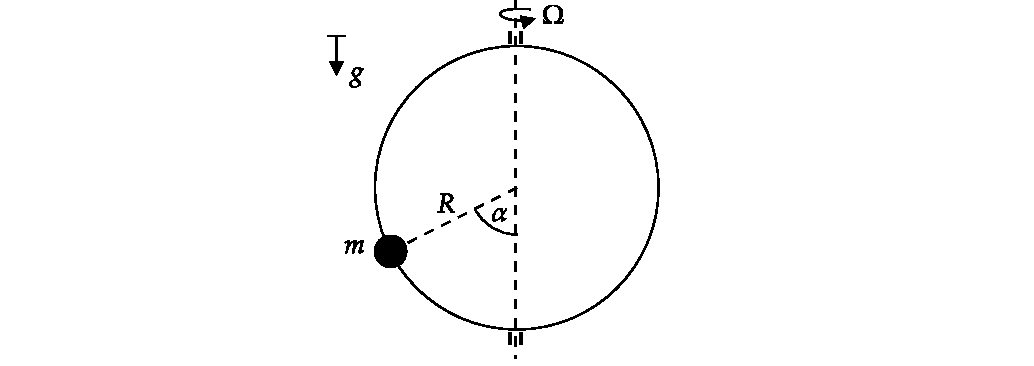
\includegraphics[scale=0.9]{Graphics/Q01D01.pdf}
	\caption{Mass on a hoop}
	\label{Q01D01}
\end{figure}
The angular velocity of the hoop is $\Omega$, the viscous friction coefficient between the hoop and the ball is $b$, and the constant of gravity in $g$. The equation of motion for the sliding ball is given by
\begin{equation*}
	mR^2 \ddot{\alpha} + bR^2 \dot{\alpha} + mR^2(g/R - \Omega^2 \cos(\alpha)) \sin(\alpha) = 0.
\end{equation*}

\begin{enumerate}[label=(\alph*)]
	\item Plot the location of equilibria of the ball as a function of the non-dimensionalized rotation parameter $\nu = R\Omega^2 /g$.
	\item Using linearization, determine the stability type of the different equilibrium branches on the plot. Identify the critical angular velocity at which a bifurcation of equilibria occurs.
\end{enumerate}

\section*{Question 2}
Consider a discrete dynamical system given by the iterated mapping
\begin{equation*}
	x_{k+1} = f(x_k), \qquad f: \mathbb{R}^n \rightarrow \mathbb{R}^n, \qquad x_k \in \mathbb{R}^n.
\end{equation*}
Assume that $x = p$ is a fixed point for the mapping, i.e., $p = f(p)$.

\begin{enumerate}[label=(\alph*)]
	\item Derive a linearized mapping of the form
	\begin{equation}\label{Q02E01}
		y_{k+1} = Ay_k
	\end{equation}
	to describe the discrete dynamics in the vicinity of the fixed point.
	\item Assume that $A$ has eigenvalues $\lambda_1, \ldots, \lambda_n \in \mathbb{C}$ with corresponding $n$ linearly independent eigenvectors $s_1, \ldots, s_n \in \mathbb{C}^n$. Show that the general solution of (\ref{Q02E01}) is of the form
	\begin{equation}\label{Q02E02}
		y_k = c_1 \varphi_1(k) + \cdots + c_n \varphi_n(k), \qquad \varphi_i(k) = \lambda_i^ks_i.
	\end{equation}
	\item Formulate a definition of stability, asymptotic stability, and instability for the $y=0$ fixed point of (\ref{Q02E01}).
	\item Using (\ref{Q02E02}), find a sufficient and necessary condition for the asymptotic stability you have defined in (c).
\end{enumerate}

\section*{Question 3}
The first three modes of a convecing fluid motion in a two-dimensional layer heated from below are described by the famous \textit{Lorenz equations}
\begin{align*}
	\dot{x} &= a(y - x), \\
	\dot{y} &= bx - y - xz, \\
	\dot{z} &= xy - cz.
\end{align*}
Here $a>0$ denotes the Prandtl number, $b>0$ is the Rayleigh number, and $c>0$ is the aspect ratio. Lorenz's original assumption is that $a > 1 + c$.

The above equations describe the evolution of the amplitudes of one velocity mode and two temperature modes. As a paradigm of chaotic dynamics, this system has inspired much of the development of the modern geometric theory of dynamical systems.

\begin{enumerate}[label=(\alph*)]
	\item Complicated dynamics arise when all possible equilibria of the system become unstable, and hence solutions cannot settle down to any simple steady state. Show that this is the case when
	\begin{equation*}
		b > \frac{a(3 + a + c)}{a - c - 1}
	\end{equation*}
	\textit{Note}: Note: A negative sign for one of the Routh-Hurwitz determinants actually implies instability, not just the lack of asymptotic stability.
	\item Solve the Lorenz equations numerically for $a=10$, $b=28$, and $c=8/3$, choosing an initial condition close to $x=y=z=0$. Plot the trajectory in three dimensions to show that it converges to a complicated surface, a \textit{chaotic attractor}.
\end{enumerate}

\section*{Question 4}
Recall from Question 1 that a ball of mass $m$ sliding on a hoop rotating with angular velocity $\Omega$ satisfies the differential equation
\begin{equation}\label{Q04E01}
	mR^2 \ddot{\alpha} + mR^2(g/R - \Omega^2 \cos(\alpha)) \sin(\alpha) = 0
\end{equation}
if there is no friction between the hoop and the mass, i.e. we assume $b=0$. 
 Assume that the parameter values are such that the lower equilibrium position of the ball is stable in linear approximation.

\begin{enumerate}[label=(\alph*)]
	\item Show that in this case, the equilibrium is also nonlinearly stable. 
	
	\textit{Hint}: Note that system (\ref{Q04E01}) is not conservative: an external torque is required to maintain the constant rotation of the hoop. As a result, the total mechanical energy of the system is not expected to work as a Lyapunov function. To find another candidate for a Lyapunov function, find a quantity that \textit{is} conserved along trajectories. Such a quantity can be found by multiplying equation (\ref{Q04E01}) by $\dot{\alpha}$ and integrating in time.
	\item Prove that the equilibrium \textit{cannot} be asymptotically stable for the nonlinear system.
	
	\textit{Hint}: use the Lyapunov function you have found in (a).
\end{enumerate}

\section*{Question 5}
Consider the damped pendulum equation
\begin{equation}\label{Q05E01}
	\ddot{x} + c\dot{x} + \sin(x) = 0.
\end{equation}

\begin{enumerate}[label=(\alph*)]
	\item Using the energy of the pendulum as a Lyapunov function, can we conclude the nonlinear asymptotic stability of the $x=0$ equilibrium ? Give detailed reasoning why.
	\item A theorem due to Krasovski states the following: Assume that $x=0$ is a fixed point for the $n$-dimensional dynamical system $\dot{x}=f(x)$. Assume that there exists a smooth scalar function $V(x)$ such that
	\begin{enumerate}[label=(\roman*)]
		\item $V(x)$ is positive definite on an open neighborhood $U$ of $x=0$
		\item $\dot{V}$ is negative semi-definite on the same neighborhood
		\item the only trajectory lying \textit{completely} in the set $S= \{ x\in U \, : \, \dot{V}=0 \}$ is the fixed point $x=0$. Then $x=0$ is asymptotically stable.
	\end{enumerate}
	Use Krasovski's theorem to conclude the asymptotic stability of the origin for (\ref{Q05E01}).
\end{enumerate}

\section*{Question 6}
Consider an $n$-degree-of-freedom holonomic mechanical system (i.e. one that has only position-dependent constraints) with generalized coordinates $q\in \mathbb{R}^n$ and generalized velocities $\dot{q}\in \mathbb{R}^n$. The total energy of the system is of the form
\begin{equation*}
	E(q, \dot{q}) = \frac{1}{2} \dot{q}^T M(q)\dot{q} + V(q),
\end{equation*}
where $M \in \mathbb{R}^{n \times n}$ is the mass matrix (symmetric ans positive definite), and $V(q)$ is the potential energy. In the absence of external forces, the associated Lagrangian equations of motion are
\begin{equation*}
	\frac{d}{dt} \frac{\partial L}{\partial \dot{q}} - \frac{\partial L}{\partial q} = 0,
\end{equation*}
where $L(q, \dot{q}) = \frac{1}{2}\dot{q}^T M(q)\dot{q} - V(q)$ is the Lagrangian of the mechanical system.

Show that if $V(q)$ admits a strict local minimum at a point $q_0$, then $q_0$ is a (nonlinearly) stable equilibrium for the mechanical system. (This result is also known as \textit{Dirichlet's Theorem} in classical mechanics).




\end{document}